\documentclass[tikz,border=8pt]{standalone}
\usetikzlibrary{arrows.meta,positioning}

\begin{document}
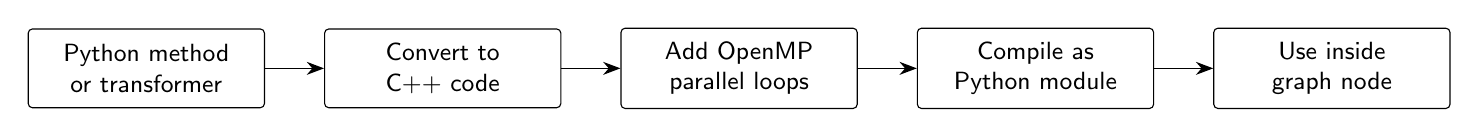
\begin{tikzpicture}[
  font=\sffamily\small,
  box/.style={
    draw=black,
    rounded corners=1.5pt,
    align=center,
    minimum width=3.0cm,
    minimum height=1.0cm,
    inner sep=5pt
  },
  arrow/.style={-{Stealth[length=2.2mm]}, line width=0.5pt}
]

\node[box] (python) {Python method\\or transformer};
\node[box, right=0.75cm of python] (convert) {Convert to\\C++ code};
\node[box, right=0.75cm of convert] (parallel) {Add OpenMP\\parallel loops};
\node[box, right=0.75cm of parallel] (compile) {Compile as\\Python module};
\node[box, right=0.75cm of compile] (graph) {Use inside\\graph node};

\draw[arrow] (python) -- (convert);
\draw[arrow] (convert) -- (parallel);
\draw[arrow] (parallel) -- (compile);
\draw[arrow] (compile) -- (graph);

\end{tikzpicture}
\end{document}
